\documentclass[serif,mathserif, 12pt]{beamer}
\usepackage{etex}
\usepackage{amsmath, amsfonts, epsfig, xspace}
\usepackage{algorithm,algorithmic}
\usepackage{pstricks,pst-node}
\usepackage{multimedia}
\usepackage[normal,tight,center]{subfigure}
\setlength{\subfigcapskip}{-.5em}
\usepackage{beamerthemesplit}
\usetheme{lankton-keynote}
\usepackage{graphicx,color}
% remove caption of figure
\usepackage[labelformat=empty]{caption}

\usepackage[none]{hyphenat} % hyphenation is ugly in slides
\usepackage{parskip}

\usepackage{relsize} % \smaller to change size

\usepackage{tikz}
\usetikzlibrary{calc}

\usetikzlibrary{arrows}

\newcommand{\TikzDraw}[2][]{
  \begin{tikzpicture}[overlay, remember picture, shift={(current page.center)}, #1]
    #2
  \end{tikzpicture}
}

\newcommand{\gridlines}{
  \TikzDraw{
    \draw[help lines,xstep=.2,ystep=.2,red!20] (current page.south west) grid (current page.north east);
    \draw[help lines,xstep=1,ystep=1,red] (current page.south west) grid (current page.north east);
    \foreach \x in {-15,-14,...,15} {
      \node [anchor=north, red] at (\x,0) {\tiny \x};
      \node [anchor=east,red] at (0,\x) {\tiny \x};
    }
  }
}

\newcommand{\DrawOnImg}[3][]
{
  \begin{tikzpicture}
    \node[anchor=south west,inner sep=0] (image) at (0,0){
      #2
    };
    \begin{scope}[x={(image.south east)},y={(image.north west)}]
      \ifthenelse{\equal{#1}{grid}}
                 {\draw[color=blue, style=dashed] (0,0) grid[xstep=.1, ystep=.1] (1.0001,1.0001);}
                 {}
                 #3
    \end{scope}
  \end{tikzpicture}
}

\usetikzlibrary{matrix}

\newcommand{\BOLD}[1]{\mathbf{#1}}
\newcommand{\BOLDG}[1]{\boldsymbol{#1}}
\newcommand{\PDIF}[2]{\frac{\partial #1}{\partial #2}}
\newcommand{\TODO}[1]{\textcolor{red}{#1}}
\newcommand{\TODOB}[1]{\textcolor{blue}{#1}}
\newcommand{\TODOG}[1]{\textcolor{green!50!black}{#1}}
\newcommand{\argmin}{\operatornamewithlimits{arg\min}}
\DeclareMathOperator{\tr}{tr}
\DeclareMathOperator{\cond}{cond}
\DeclareMathOperator{\ST}{s.t.}
\DeclareMathOperator{\diag}{diag}
\DeclareMathOperator{\Div}{div}

\author[Jiong Chen]{Jiong Chen}

\title[\hspace{2em}\insertframenumber/\inserttotalframenumber]{Regularized Kelvinlets: Sculpting Brushes based on Fundamental Solutions of Elasticity}
\date{November 2, 2017}

% \institute{Zhejiang University}

\begin{document}

\maketitle

\begin{frame}
  \frametitle{Motivation}
  \begin{itemize}
  \item Digital sculpting for modeling and animation.
    \visible<2-> {\item Common modeling primitives}
    \visible<2-> {
      \begin{itemize}
      \item[-] grab, scale, twist, pinch
      \end{itemize}
      }
    \visible<3-> {\item Geometric approach: natural deformation}
    \visible<4-> {\item Physically based approach: interactive performance}
    \TikzDraw {
      \visible<1-> {
        \node at (0, -2.6) {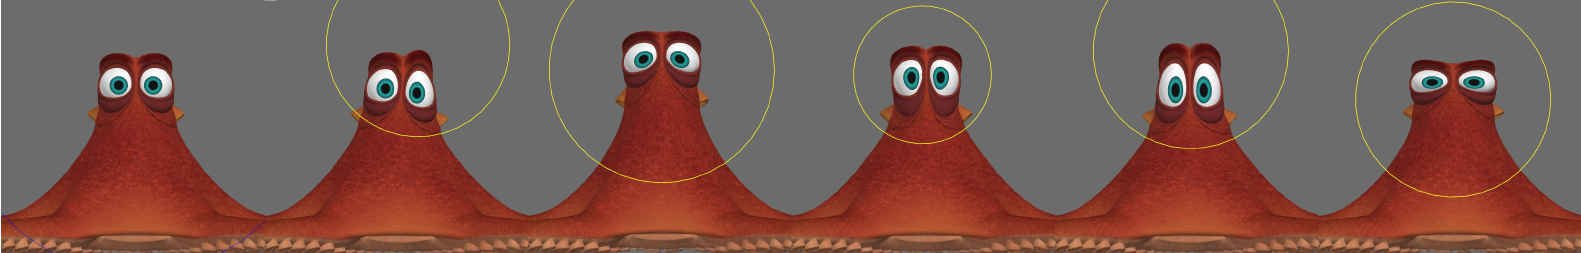
\includegraphics[width=0.95\textwidth]{img/digital_sculpting}};
      }
      \visible<3-> {
        \draw[red, thick] (-0.6, -0.7)--(3.2, -0.7);
      }
      \visible<4-> {
        \draw[red, thick] (0.6, -1.5)--(5.2, -1.5);
      }
    }
  \end{itemize}
  %\gridlines
\end{frame}

\begin{frame}
  \frametitle{Key Ideas}
  \begin{itemize}
  \item Goal
    \begin{itemize}
    \item[-] Interactive, physically plausible deformation with
    specific editing primitives
    \end{itemize}
    \pause
  \item Tools: Fundamental solutions to the linear elasticity
    \begin{itemize}
    \item[-] free of geometric discretization
    \item[-] computational efficient
    \item[-] low memory cost
    \end{itemize}
  \end{itemize}  
\end{frame}

\begin{frame}
  \frametitle{Background}
  \begin{itemize}
  \item Small train
    \begin{equation*}
      \epsilon = \frac{1}{2}(\nabla u^T + \nabla u)
    \end{equation*}
  \item Elastic potential
    \begin{equation*}
      E(u) = \mu\|\epsilon\|_F^2 + \frac{\lambda}{2}\tr(\epsilon)^2
    \end{equation*}
  \item Another formulation
    \begin{equation*}
      E(u) = \frac{\mu}{2}\|\nabla u\|^2 + \frac{\mu}{2(1-2\nu)}\|\nabla \cdot u\|^2
    \end{equation*}
  \end{itemize}
\end{frame}

\begin{frame}
  \frametitle{Background}
  \begin{itemize}
  \item Navier-Cauchy equation
    \begin{equation*}
      \mu \Delta u + \frac{\mu}{1-2\nu}\nabla(\nabla \cdot u) + b = 0
    \end{equation*}
    \pause
  \item With $b(x) = f\delta(x-x_0)$
    \begin{equation*}
      u(r) = \left[ \frac{a-b}{\|r\|}I+ \frac{b}{\|r\|^3}rr^T\right]f = K(r)f, \quad r = x-x_0
    \end{equation*}
  \end{itemize}
  \TikzDraw {
    \visible<3> {
    \node at (0, -3) {
      \textcolor{red}{\emph{Kelvin state or Kelvinlets}}
    };
    }
  }
\end{frame}

\begin{frame}
  \frametitle{Notes on Derivation}
  \begin{itemize}
  \item Some assumptions on $u$
    \begin{equation*}
      u = \frac{1}{2\mu}\nabla \phi
    \end{equation*}
    \pause
  \item Papkovich-Neuber solution
    \begin{equation*}
      \begin{split}
        &\BOLD{u} = \frac{1}{2\mu}(-4(1-\nu)\BOLDG{\psi} +\nabla (\BOLD{r}\cdot \BOLDG{\psi}+\phi)), \\
        &\nabla^2 \BOLDG{\psi} = \BOLD{0}, \nabla^2 \phi = 0
      \end{split}      
    \end{equation*}
  \end{itemize}
\end{frame}

\begin{frame}
  \frametitle{3D Regularized Kelvinlets}
  \begin{itemize}
  \item Smoothed body load
    \begin{equation*}
      b(r) = f\rho_\epsilon (r)
    \end{equation*}
  \item density function
    \begin{equation*}
      \rho_\epsilon(r) = \frac{15\epsilon^4}{8\pi}\frac{1}{r_\epsilon^7}, r_\epsilon = \sqrt{r^2+\epsilon^2}
    \end{equation*}
  \item Regularized Kelvinlets
    \begin{equation*}
      \begin{split}
      &u_\epsilon(r) = \left[\frac{a-b}{r_\epsilon}I+\frac{b}{r_\epsilon^3}rr^T+\frac{a}{2}
        \frac{\epsilon^2}{r_\epsilon^3}I\right]f = K_\epsilon(r)f \\
      &u_\epsilon(0) = \bar u \Rightarrow u_\epsilon(r) = c\epsilon K_\epsilon(r) \bar u
      \end{split}
    \end{equation*}
  \end{itemize}
  \TikzDraw {
    \node at (4.5, 0) {
      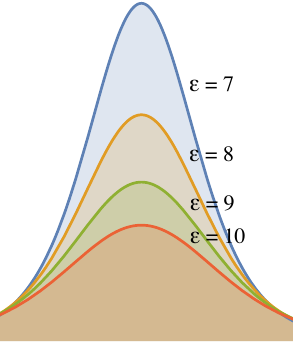
\includegraphics[width=0.2\textwidth]{img/rho}
    };
  }
\end{frame}

\begin{frame}
  \frametitle{Slow Spatial Decay}
  \TikzDraw {
    \visible<1> {
      \node at (0, 0) {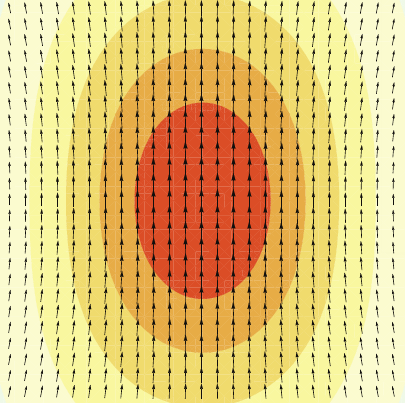
\includegraphics[width=0.6\textwidth]{img/single_scale}};
      \node at (0, -3.5) {$\epsilon$};
    }
    \visible<2> {
      \node at (0, 0) {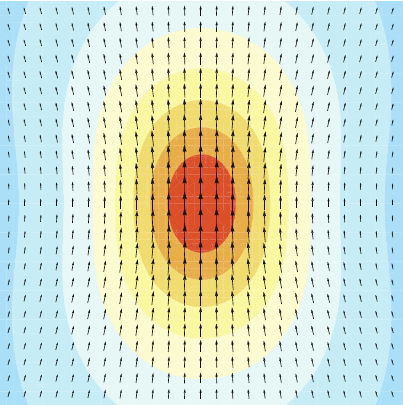
\includegraphics[width=0.6\textwidth]{img/half_scale}};
      \node at (0, -3.5) {$0.5\epsilon$};
    }
  }
\end{frame}

\begin{frame}
  \frametitle{Slow Spatial Decay}
  \begin{itemize}
  \item Richardson extrapolation
    \begin{equation*}
      A(h) = A^* + \mathcal{O}(h^n) = A^* + Ch^n + \mathcal{O}(h^{n+1})      
    \end{equation*}
    \pause
  \item Consider $R(h, k)$
    \begin{equation*}
      \begin{split}
      &R(h, k) = \frac{k^n}{k^n-1}A(h) -\frac{1}{k^n-1}A(kh) \\
      \visible<2-> {
        &=\frac{k^n(A^*+Ch^n+\mathcal{O}(h^{n+1}))-(A^*+Ck^nh^n+\mathcal{O}(h^{n+1}))}{k^n-1} \\
        &=A^* + \mathcal{O}(h^{n+1})
      }
      \end{split}
    \end{equation*}
  \end{itemize}
\end{frame}

\begin{frame}
  \frametitle{Slow Spatial Decay}
    \begin{itemize}
  \item Asymptotic analysis $K_\epsilon(r)\rightarrow \infty$
    \begin{equation*}
    C_1(\hat r)\textcolor{red}{\frac{1}{r}}+C_3(\hat r) \textcolor{red}{\frac{\epsilon^2}{r^3}}
    +C_5(\hat r)\textcolor{red}{\frac{\epsilon^4}{r^5}}+\mathcal{O}(\textcolor{red}{\frac{1}{r^7}}),~~\hat r = r/\|r\|
    \end{equation*}
    \pause
  \item \emph{Compound brushes to cancel the heading terms}
  \end{itemize}
\end{frame}

\begin{frame}
  \frametitle{Multi-scale Extrapolation}
  \begin{itemize}
    \visible<1-> {\item Bi-scale extrapolation
    \begin{equation*}
      u_{\epsilon_1, \epsilon_2}(r) = \left(K_{\epsilon_1}(r)-K_{\epsilon_2}(r)\right)f
    \end{equation*}
    }
    \visible<2-> {\item Tri-scale extrapolation
    \begin{equation*}
      \begin{split}
        &u_{\epsilon_1, \epsilon_2, \epsilon_3} = (w_1K_{\epsilon_1}(r)+
        w_2K_{\epsilon_2}(r)+w_3K_{\epsilon_3}(r))f  \\}
        \visible<3-> {&\left(\sum_i w_i\right)C_1(\hat r)\frac{1}{r}
        +\left(\sum_i w_i\epsilon_i^2\right)C_3(\hat r)\frac{\epsilon^2}{r^3}+\mathcal{O}(\frac{1}{r^5}) \\
        &w_1 = 1, w_2 = -(\epsilon_3^2-\epsilon_1^2)/(\epsilon_3^2-\epsilon_2^2),
        w_3 = (\epsilon_2^2-\epsilon_1^2)/(\epsilon_3^2-\epsilon_2^2)
        }
      \end{split}
    \end{equation*}
  \end{itemize}
\end{frame}

\begin{frame}
  \frametitle{Multi-scale Extrapolation}
  \begin{figure}
    \centering
    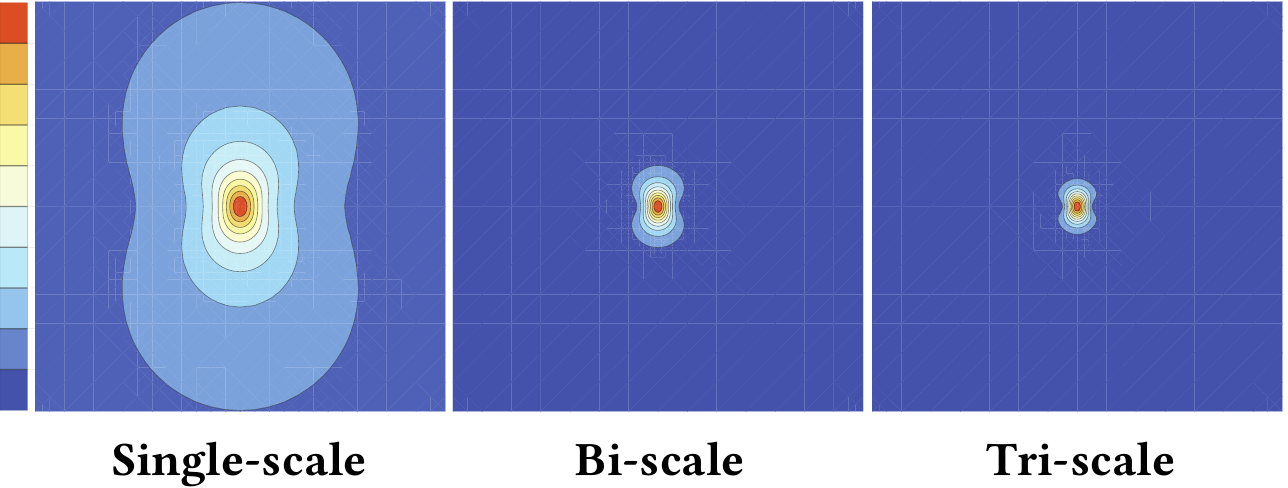
\includegraphics[width=\textwidth]{img/single_bi_tri}
  \end{figure}
\end{frame}

\begin{frame}
  \frametitle{Extension to Affine Loads}
  \TikzDraw {
    \visible<1-> {\node at (0, 2.5) {
      \parbox[t]{\textwidth} {
        \begin{equation*}
          u_\epsilon(r) = u_\epsilon(\bar u \cdot r)
        \end{equation*}
      }
      };
    }
    \visible<2-> {
    \node at (0, 0) {
      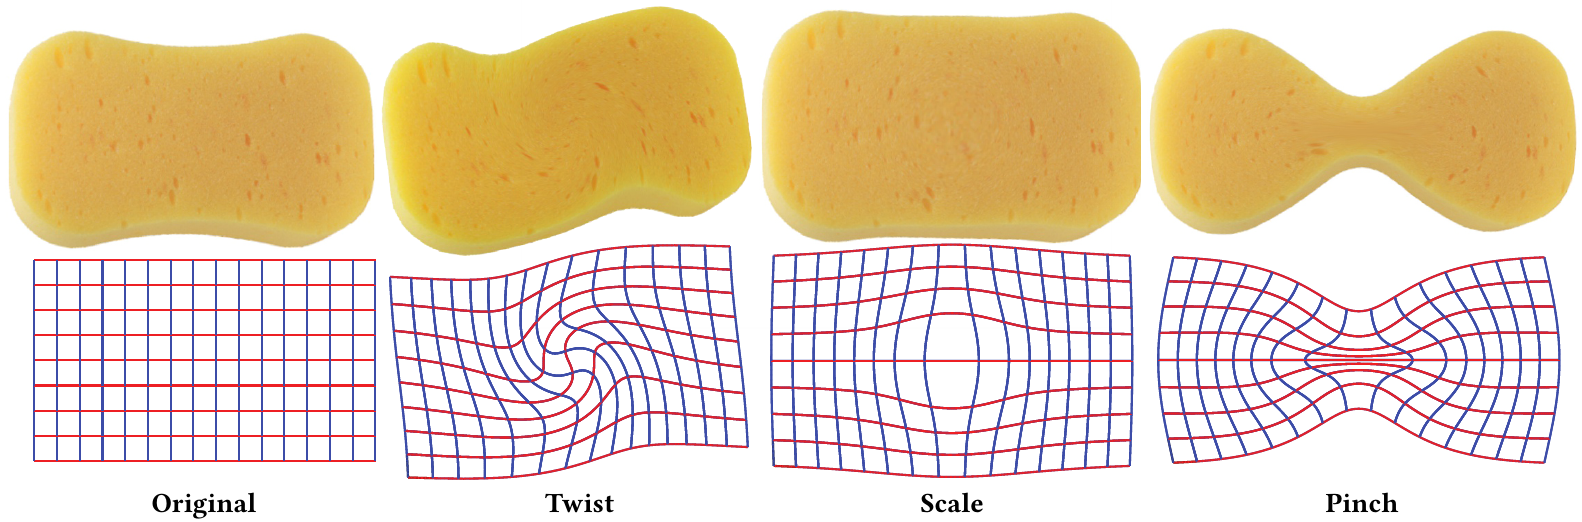
\includegraphics[width=\textwidth]{img/affine_loads}
    };
    }
    \visible<3-> {
    \node at (0, -2.7) {
      \parbox[t]{\textwidth} {
        \begin{equation*}
          u_\epsilon(r) = u_\epsilon(F r)
        \end{equation*}
      }
    };
    }
  }
\end{frame}

\begin{frame}
  \frametitle{Extension to Affine Loads}
  \begin{itemize}
  \item Directional derivative of Navier-Stokes equation
    \begin{equation*}
      \begin{split}
      0 &= g\cdot \nabla \left(\mu \Delta u_\epsilon + \frac{\mu}{1-2\nu}\nabla(\nabla \cdot u_\epsilon) +b\right)\\
      &= \mu \Delta (g\cdot \nabla u_\epsilon) + \frac{\mu}{1-2\nu}\nabla (\nabla \cdot
      (g\cdot \nabla u_\epsilon)) + g\cdot \nabla b \\
      \\
      \visible<2> {&\tilde b(r) = g\cdot \nabla b(r) = g\cdot \nabla (f\rho_\epsilon(r)) \\
        &\tilde u_\epsilon(r) = g\cdot \nabla u_\epsilon(r) = g\cdot \nabla (K_\epsilon(r)f)
        }
      \end{split}
    \end{equation*}
  \end{itemize}
  \TikzDraw {
    \visible<3> {
      \node at (-0.74, -1.6) {
        \parbox[t]{\textwidth} {
          \begin{equation*}
            \begin{split}
              &\tilde b(r) = g\cdot \nabla b(r) = \textcolor{red}{e_j}\cdot \nabla (\textcolor{red}{e_i}\rho_\epsilon(r)) \\
              &\tilde u_\epsilon(r) = g\cdot \nabla u_\epsilon(r) = \textcolor{red}{e_j}\cdot
              \nabla (K_\epsilon(r)\textcolor{red}{e_i})
            \end{split}
          \end{equation*}
        }
      };
    }
    \TikzDraw {
      \visible<2-> {
      \draw[red, thick] (-2.8, -0.1)--(-1.2, -0.1);
      \draw[red, thick] (1.7, -0.1)--(3.4, -0.1);
      \draw[blue, thick] (4.0, -0.1)--(5.0, -0.1);
      }
    }
  }
\end{frame}

\begin{frame}
  \frametitle{Extension to Affine Loads}
  \begin{itemize}
  \item By combining all pair of $(e_i, e_j)$
    \begin{equation*}
      \begin{split}
        \tilde u_\epsilon(r) &= \textcolor{red}{\sum_{ij} F_{ij} e_j \cdot\nabla (K_\epsilon(r) e_i)} = \nabla K_\epsilon(r): F \\
        \visible<2-> {
        &= -a\left(\frac{1}{r_\epsilon^3}+\frac{3\epsilon^2}{2r_\epsilon^5}\right)Fr \\
          &+ b\left(\frac{1}{r_\epsilon^3}(F+F^T+\tr(F)I)-\frac{3}{r_\epsilon^5}(r^TFr)I\right)r
          }
      \end{split}      
    \end{equation*}
  \end{itemize}
\end{frame}

\begin{frame}
  \frametitle{Extension to Affine Loads}
  \begin{itemize}
  \item Twisting: $F = [q]_\times$
    \begin{equation*}
      u_\epsilon(r) = -a(\frac{1}{r_\epsilon^3}+\frac{3\epsilon^2}{2r_\epsilon^5})q\times r
    \end{equation*}
  \item Scaling $F = sI$
    \begin{equation*}
      u_\epsilon(r) = (2b-a)(\frac{1}{r_\epsilon^3}+\frac{3\epsilon^2}{2r_\epsilon^5})(sr)
    \end{equation*}
  \item Pinching, $F^T = F, \tr(F) = 0$
    \begin{equation*}
      u_\epsilon(r) = \frac{2b-a}{r_\epsilon^3}Fr - \frac{3}{2r_\epsilon^5}(2b(r^TFr)I +a\epsilon^2 F)r
    \end{equation*}
  \end{itemize}
\end{frame}

\begin{frame}
  \frametitle{Constrained Deformation}
  \begin{itemize}
  \item Displacement constraints
    \begin{equation*}
      \begin{split}
        &u(x) =\sum_i^n K_{\epsilon_i}(x-x_i)f_i \\
        &
        \begin{pmatrix}
          0 \\ \bar u_n
        \end{pmatrix}
        =
        \begin{pmatrix}
          K_{pp}& K_{pn}\\
          K_{np}& K_{nn}
        \end{pmatrix}
        \begin{pmatrix}
          f_p \\ f_n
        \end{pmatrix}
      \end{split}      
    \end{equation*}
  \end{itemize}
\end{frame}

\begin{frame}
  \frametitle{Results}
  \TikzDraw {
   \visible<1-> {
     \node at (0, 0) {
       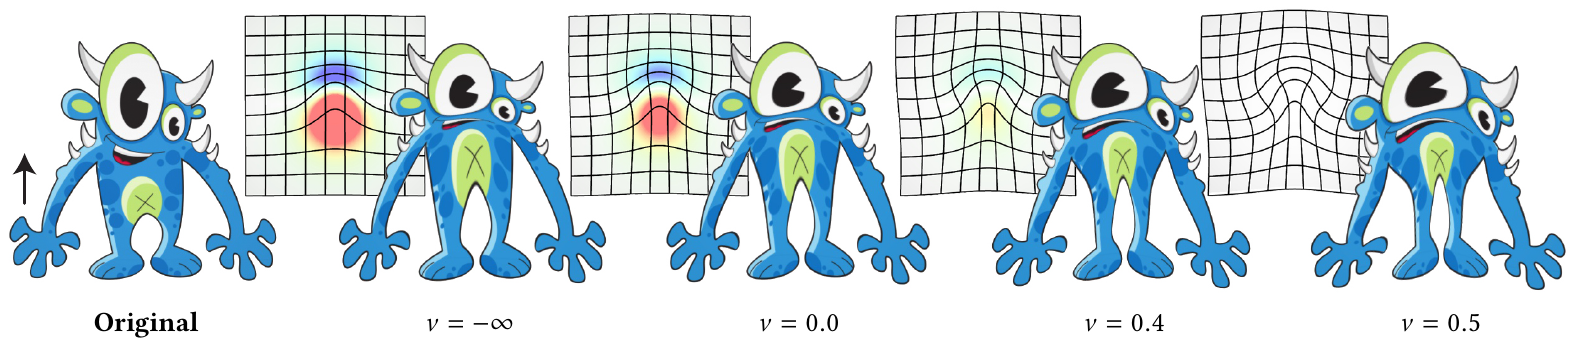
\includegraphics[width=\textwidth]{img/area_preserving}
     };
   }
   \visible<2-> {
     \node at (0, 0) {
        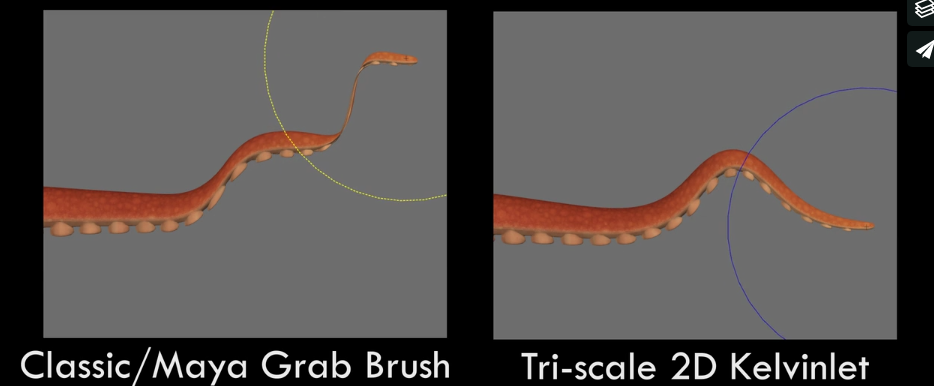
\includegraphics[width=\textwidth]{img/comparison}
     };
   }
  }
\end{frame}

\begin{frame} 
  \TikzDraw {
    \node at (0, 0.5) {\Huge{Thanks!}};
  }
  %\gridlines
\end{frame}

\end{document}
